%!TEX root = ../TTK4550-MHT.tex

\section{Survey of multi-target tracking methods}
\label{sec:survey}
The aim of this section is to give the reader a brief overview of tracking as a problem and a feeling for the most popular methods, their assumptions and strong and weak properties as seen from an two dimensional maritime anti collision perspective.

\subsection{Tracking}
Tracking of an object (\gls{target}) is the process of estimating its state (i.e. position and velocity) based on discrete \glspl{measurement} from an observation system. An observation system can be a \gls{radar}, sonar or any other sensor that passively or actively detects objects within an area or volume. Any observation system will be prone to noise, both in form of internal noise and external noise from the environment. This noise will, in varying degree, cause false \glspl{measurement} that the tracking system must take care of. These false \glspl{measurement} are often refereed to as \gls{clutter}. 

\subsection{Tracking system}
A tracking system can be interpreted as either the complete system from the signal processing level to the finished tracks, or as I define it in this text: \emph{A system that process consecutive \glspl{measurement} from an observation system and collects \glspl{measurement} from the same \gls{target} into tracks or initiate new tracks.} A track is a subset of all the \glspl{measurement} from the observation system that is believed to originate from the same \gls{target}. The challenge knowing which \gls{measurement} originating from which (real) \gls{target} is the core at any tracking system. This association problem is non-trivial even under ideal situations, and the addition of spurious \glspl{measurement} and missed \glspl{target} only increases the complexity.

There has been developed a large variety of methods to solve this association problem, and most of them have several sub-variants. In the following subsections, some of the most common and popular methods will be presented.

\subsection{Nearest Neighbour Filter}
\label{sec:nn}
The \gls{nnf} is the simplest approach in tracking, where one always selects the closest neighbour as the consecutive \gls{measurement} in the track, where the distance is the Euclidean distance (\ref{eq:euclidian_distance}).
\begin{equation}
\left[ (z_k-z_{k-1}) \cdot (z_k-z_{k-1}) \right]^{1/2}
\label{eq:euclidian_distance}
\end{equation}
This approach suffers from being very vulnerable to clutter and dense \gls{target} scenarios. It can be somewhat improved by estimating an a-priori state through a Kalman Filter and selecting the nearest neighbour to the estimate. This extension is sometimes refereed to as \gls{nnsf} \cite{Bar-Shalom1998} and also differs in that it used the Mahalanobis distance (\ref{eq:mahalanobis_distance}) which is a measure of the distance from a \gls{measurement} to a distribution.
\begin{equation}
\left[ z_k - \hat{z}_{k} \right]^T S(k+1)^{-1} \left[ z_k - \hat{z}_{k} \right]
\label{eq:mahalanobis_distance}
\end{equation}
Under the standard assumption that each \gls{target} can at maximum generate one \gls{measurement}, the \gls{nnf} and \gls{nnsf} are both single-\gls{target} methods in the way that they may assign the same \gls{measurement} to more than one track. They can, however, be expanded to multi-\gls{target} variants by formulating the problem as a global least squares integer optimization problem, often called \gls{gnnf}. With this extension, the \gls{nnsf} is almost becoming a zero-scan multi hypothesis tracker, in the sense that it seeks to select the optimal combination of mutual exclusive measurement-to-track associations while only looking at the most recent \gls{scan}. \gls{nnf}, \gls{nnsf} and \gls{gnnf} can be viewed as non-probabilistic models, as they do not assume specific models for noise, clutter, false alarm rate or similar.

\subsection{Probabilistic Data Association Filter}
\label{pdaf}
\gls{pdaf} is a \emph{single-target} Bayesian association filter which is based on single scan probabilistic analysis of \glspl{measurement}. The \gls{target} is assumed initialized and modelled by (\ref{eq:kalman_model}). At each scan, the algorithm calculates the association probabilities for all the \glspl{measurement} inside a validation gate, with the assumption that at most one of the \glspl{measurement} inside the validation gate is the true \gls{target}. This leads to the state update equation (\ref{eq:pdaf_state_update}) where the current state is updated with a combined innovation.
\begin{equation}
\begin{split}
\V{\nu}_k &\triangleq \sum\limits_{i=1}^{m_k} \beta_k^i \V{\tilde{y}}_k^i \\
\V{\hat{x}}_{k|k} &= \V{\hat{x}}_{k|k-1} + \M{K}_k \V{\nu}_k
\end{split}
\label{eq:pdaf_state_update}
\end{equation} 
where
\begin{equation*}
\begin{split}
	\beta_k^i	&= \text{the probability of measurement $z^i$ beeing the correct one} \\
	\V{\tilde{y}}_k^i &= \V{z}_k^i - \V{\hat{z}}_k^i \hspace{5mm}	\text{the measurement innovation for mesurement $i$ at time step k} \\
	\M{K}_k 	&= \text{the Kalman Gain for the k-th time step} \\
	\V{x}_k 	&= \text{target state}
\end{split}
\end{equation*}
\begin{wrapfigure}[20]{R}{0.5\textwidth}
\centering
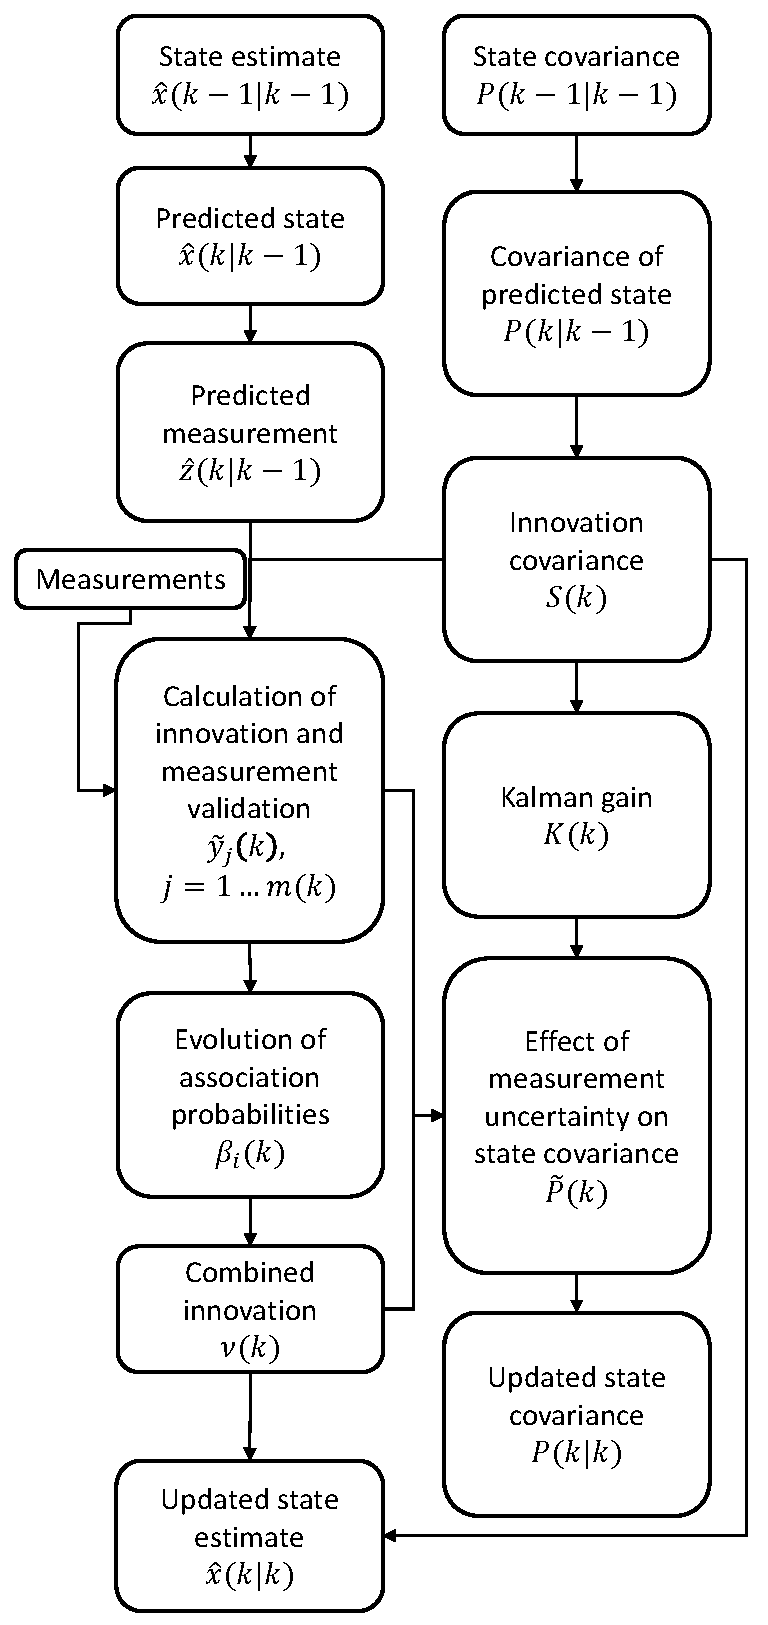
\includegraphics[height = .6\textheight]{pdaf-flowchart}
\caption{\gls{pdaf} flowchart \cite{Bar-Shalom1998}}
\label{fig:pdaf_flowchart}
\end{wrapfigure}
PDAF is computationally modest (approximate 50\% more computationally demanding than a Kalman Filter \cite{Bar-Shalom1998} p.163) and have good results in an environment with up to about 5 false \gls{measurement} in a $4\sigma$ validation region \cite{Bar-Shalom1998}. PDAF does not include track initialization and assumes that at most one \gls{measurement} can originate from an actual \gls{target}. It also assumes that clutter is uniformly distributed in the \gls{measurement} space and that the \glspl{target} history is approximated by a Gaussian with a calculated mean and covariance.

\gls{pdaf} can be used in multi-\gls{target} scenarios, but only as multiple copies of the single-\gls{target} filter \cite{Fortmann1983}. \gls{pdaf} can suffer from track coalescence, which is a phenomenon that merges two tracks into one. This coalescence occurs when two \glspl{target} have similar paths, and the resulting tracks will be an "average" of the two (actual) tracks. There has been done some work to overcome this coalescence \cite{Blom2000}.

\subsection{Joint Probabilistic Data Association Filter}
\label{sec:jpdaf}
The \gls{jpdaf} is a \emph{multi-\gls{target}} extension of the Probabilistic Data Association Filter in which joint posteriori association probabilities are calculated for every \gls{target} at each scan. Both \gls{pdaf} and \gls{jpdaf} use the same weighted sum (\ref{eq:pdaf_state_update}), the key difference is the way the weight $\beta_i^j$ is calculated. Whereas \gls{pdaf} treats all but one \gls{measurement} inside its validation region as clutter, in \gls{jpdaf} the \glspl{target} which interacts (one cluster) are treated as connected and the connected $\beta_i^j$s are computed jointly across the cluster set with a given set of active \glspl{target} inside the cluster. The probability of a \gls{measurement} $i$ belonging to a \gls{target} $j$ is \cite{Fortmann1983}
\begin{equation}
\begin{split}
\beta_i^j &= \sum_{\chi} P\{ \chi | Y^k \} \hat{\omega}_{ij}(\chi) \\
\beta_0^j &= 1 - \sum_{i=1}^{m_k} \beta_i^j
\end{split}
\end{equation}
where
\begin{equation}
P\{\chi|Y^k\} = \frac{C^\phi}{c} 
				\prod_{i:\tau_i=1} \frac{\mathrm{exp}[-\frac{1}{2}(\V{\tilde{y}_i^{j}})^T S_{j_i}^{-1}(\V{\tilde{y}_i^{j}})]}{(2\pi)^{M/2} |S_{j_i}|^{1/2}}
				\prod_{j:\delta_j=1} P_D^j
				\prod_{j:\delta_j=0} (1 - P_D^j)
\end{equation}%
Where 
\begin{equation*}
\begin{split}
	\beta_i^j			&= \text{the probability that measurement $i$ belongs to target $j$} \\
	\beta_0^j 			&= \text{the probability that no measurement belongs to target $j$} \\
	\chi 				&= \bigcap\limits_{i=1}^{m_k} \chi_{i j_i} \quad \text{All feasible events} \\
	Y^k 				&= \text{all candidate measurements up to and included time $k$} \\
	\hat{\omega}_{ij}	&=	\begin{cases}
								1, \text{if } \chi_{ij} \text{ occurs} \\ 
								0, \text{otherwise} 
							\end{cases} \\
	m_k					&= \text{number of measurements in scan $k$}
\end{split}
\end{equation*}
Since the \gls{jpdaf} is calculating joint probabilities for all the combinations of \gls{measurement} associations in the cluster, the computation demand is growing exponentially with the numbers of tracks and \glspl{measurement} in the cluster. A real time implementation of the \gls{jpdaf} has been developed and patented by QinetiQ \cite{QinetiQ2003}, and described in \cite{Horridge}.

\gls{jpdaf} also suffers from the same coalescence problem as \gls{pdaf}. Seen from a anti-collision perspective, track coalescence is highly undesirable. An improvement to the \gls{jpdaf} has been proposed by \cite{Blom2000}.

Since \gls{jpdaf} is using all the \glspl{measurement} inside the gate for each track, one \gls{measurement} can be used to update more than one track if is within more that one gate.

\subsection{Multi Hypothesis Tracker}
\label{sec:mht}
\gls{mht} is a decision logic which generates and maintains alternative hypotheses when new \gls{measurement} are received and within the gate. By making several possible hypotheses, the decision in which \gls{measurement} to choose can be propagated into the future when more information is available. Each hypothesis is given a \gls{score} or probability as a measure of the goodness of the \gls{measurement}, which are accumulated to evaluate the combinations of consecutive \glspl{measurement}.

In contrast to \gls{pdaf} and \gls{jpdaf} methods which in general will estimate an "average" of two closely spaced tracks as the true track (coalesce), \gls{mht} methods split when in doubt. The idea of using multiple hypotheses was first introduced by Singer. et al. \cite{Singer1974}, but the first complete algorithm was presented by Reid \cite{Reid1979}, where a \gls{homht} was developed. Following this, a \gls{tomht} was proposed in \cite{Kurien1990} and the \gls{score} function for \gls{mht} was later deduced and discussed by \cite{Bar-Shalom2007} since no explicit track-score function were given in \cite{Kurien1990}. \gls{mht} is, in the same way as \gls{pdaf}/\gls{jpdaf}, developed under the assumption that at most one \gls{measurement} can originate from each \gls{target} in each scan, and that a \gls{target} does not necessary show on every scan (\gls{Pd} less than 1).

If extracting the \gls{map} hypothesis from a \gls{mht}, apparent inconsistency in the output to the user can appear whenever a new set of \glspl{measurement} are received since all association $N$ time-steps back are reconsidered. If this is unwanted, an alternative representation is to output the N-best tracks and display them to the user in a way that visualises the probability. A third, and still not fully resolved option, is to output a weighted average of the tracks along with the covariance of the average.

The \gls{mht} approach to tracking and data association was by many for a long time dismissed because of its computationally large cost. The dramatic increase in computational capability from the 1980´s to the late 2010´s have however lead to a new spring for \gls{mht} with an increasing interest for use in tracking system. In 2004 Blackman stated \say{Multiple hypothesis tracking is generally accepted as the preferred method for solving the data association problem in modern multiple \gls{target} tracking system}\cite{Blackman2004}. Already in 2001 did Blackman publish a demonstration that \gls{mht} is capable of real-time demands \cite{Blackman2001}.

There are two main approaches to \gls{mht}, \gls{homht} and \gls{tomht}.

\subsubsection{Hypothesis Oriented MHT}
\gls{homht} or \gls{momht} is a tracking approach where direct probabilities of global joint measurement-to-target association hypothesis are calculated. The algorithm initiates tracks and handles missing \glspl{measurement}, it has a recursive nature and allows for clustering for quicker computation.

When a new set of \glspl{measurement} is received, Reid´s method defines a set of hypotheses, each containing a complete set of associations of the existing tracks and new \glspl{measurement}. By defining the hypotheses in this way, they become compatible in the sense that one and only one is the true hypothesis. When the next set of \glspl{measurement} arrives, each of the current hypotheses are expanded with all measurement-to-track assignments for the new \glspl{measurement}. This way, the hypotheses will keep their compatibility.

When evaluating the alternative hypotheses, each is assigned a probability. This probability takes into account the false-alarm statistics of the measurement system, the expected density of \glspl{target} and clutter and the accuracy of the \gls{target} estimates. The probability of each data association hypothesis was in \cite{Reid1979} expressed as (\ref{eq:homht_probability}).
\begin{equation}
P_i^k = \frac{1}{c} P_D^{N_{DT}}(1-P_D)^{(N_{TGT}-N_{DT})} \beta_{FT}^{N_{FT}} \beta_{NT}^{N_{NT}} \left[ \prod_{m=1}^{N_{DT}} N(\V{Z_m}-\M{H}\V{\bar{x}},\M{B}) \right] P_g^{k-1}
\label{eq:homht_probability}
\end{equation}
where 
\begin{equation*}
\begin{split}
	P_i^k		&= \text{the probability of hypothesis $\Omega_i^k$ given measurements up through time $k$} \\
	P_D 		&= \text{the probability of detection} \\
	\beta_{FT} 	&= \text{the density of targets} \\ 
	\beta_{NT}	&= \text{the density of previously unknown targets that have been detected} \\
	N_{DT} 		&=	\text{number of designated target} \\
	N_{FT} 		&= \text{the number of false targets} \\
	N_{NT} 		&= \text{the number of new targets} \\
	N_{TGT} 	&= \text{is the number of targets} \\
	\V{Z_m} 	&= \text{the m-th measurement in the current scan} \\
	\M{H} 		&= \text{the observation matrix} \\
	\M{B} 		&= \text{the measurement covariance}
\end{split}
\end{equation*}
As with all \gls{mht} algorithms, it is crucial to prune the hypothesis tree to avoid an infinite memory and computational cost. In \cite{Reid1979}, several pruning techniques are utilized, were the most important one is probably the procedure to remove all hypotheses with probability below a threshold. A second technique that were proposed in \cite{Reid1979} is to merge hypotheses with the last N data scans in common, where he also argues for the importance of preserving earlier rather than later hypotheses. 

The initialization of tracks is done through the probabilities of each hypothesis, where a hypothesis would go from a tentative track to a confirmed track when the probability of that hypothesis exceeds i.e. $99 \%$. By treating all new \gls{measurement} as tentative \glspl{target}, and calculate their joint probability using information such as density of false \glspl{target}, density of new \glspl{target} and probability of detection and thresholding this, the algorithm has an advanced build-in initialization mechanism.

\subsubsection{Track Oriented MHT}
\label{subsec:tomht}
\gls{tomht} is a "bottom-up" approach where the tracks are assumed initialized, and for each scan the track splits whenever there are more than one feasible \gls{measurement} in the validation region (in addition to the \gls{no-measurement hypothesis}). This give rise to a track tree, as in Figure \ref{fig:hyp-tree}, where each initialized track has a root node and multiple branches, were each level represents a scan. A hypothesis is now a set of compatible tracks, with minimum and maximum one track from each track tree, were a hypothesis' \gls{score} is the sum of its \glspl{track} \gls{score}. Tracks are compatible if they do not share any \glspl{measurement}. The optimal hypothesis is the hypothesis with the highest \gls{score}.

In the special case were each track tree does not share any \glspl{measurement} (single \gls{target} situation), the optimal track is the leaf node with the highest \gls{score}, which can be found by a traversal of the tree in linear time \cite{Tarjan1971}. However, when a \gls{measurement} is assigned to two or more \glspl{target}, the problem of selecting the optimal combination of tracks becomes a multi dimensional assignment problem, since the best hypothesis from each track tree might be mutual exclusive.

New \glspl{track hypothesis} are generated from the filtered estimate from a Kalman Filter, and a \gls{score} is calculated for instance using (20) from \cite{Bar-Shalom2007}. Both \cite{Bar-Shalom2007} and  \cite{Blackman2004} suggest that modern tracking system could improve performance in certain scenarios by using an \gls{imm} approach in stead of a single Kalman Filter. However, this would inevitably increase the computatinal complexity. Following the addition of new track hypotheses, the tracks are divided into clusters, in which tracks with common \glspl{measurement} are grouped. The clusters can then be analysed as standalone global problems to find the best possible combination of (possibly mutual exclusive) \gls{measurement} associations. \gls{lp} and \gls{ilp} based methods as proposed by \cite{Storms2003} can be used to find the best combinations of newly created track hypotheses in accordance to the assumption that a \gls{measurement} only can be assigned to one \gls{target} and that one \gls{target} can maximally create one \gls{measurement}.

To limit the size of the \gls{track hypothesis tree}, various pruning schemes have been developed. The maybe single most important pruning technique is the N-scan pruning, also known as N-scan sliding window. This is a simple technique for limiting the size of the track tree and the following number of leaf nodes. The pruning is done by selecting the node that is N levels higher that the current best leaf node as new root node.

One of the largest drawback with the \gls{tomht} approach is the difficulty of track initialization. This is because \gls{tomht} normally only considers \glspl{measurement} that are within any (already initialized) \glspl{target} \gls{gate}, and automatically discards the unused \glspl{measurement} in order to limit the computation time. An alternative could be to treat all unused measurements an new targets. This would however increase the computational demand and runtime considerably. The most common approach to add track initialization to \gls{tomht} is to run a separate initialization algorithm in parallel with the tracking loop. This initialization method can be chosen freely, and some popular alternatives are; a dedicated \gls{homht} running on all or the unused \glspl{measurement} from the main loop, a N-of-M method that can be based on either nearest neighbour or \gls{pdaf}/\gls{jpdaf} or simply a manual initialization by the user. The options for this aiding module are endless, and the specific situation will influence the choice of method.